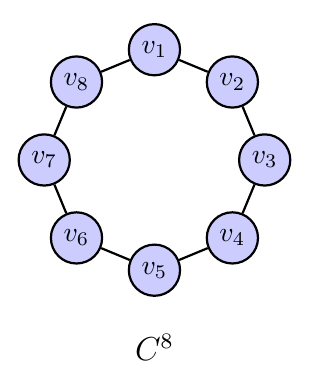
\begin{tikzpicture}[
  baseline=0pt,
  scale=0.7,
  vnode/.style={circle, draw=black, fill=blue!20, thick, inner sep=0pt, minimum size=6.5mm},
  edge/.style={thick, draw=black}
]
  \useasboundingbox (-2.3,-3.7) rectangle (2.3,2.4);

  % Vértices en radio 2.0 cm (v1 a 90°, aumentando en sentido horario)
  \foreach \i in {1,...,8} {
    \pgfmathsetmacro{\ang}{90 - (\i-1)*360/8}
    \node[vnode] (v\i) at (\ang:2.0) {$v_\i$};
  }

  % Aristas del ciclo C^8
  \draw[edge] (v1) -- (v2) -- (v3) -- (v4) -- (v5) -- (v6) -- (v7) -- (v8) -- (v1);

  % Etiqueta inferior en tamaño normal
  \node at (0,-3.4) {\large{$C^8$}};
\end{tikzpicture}
